\documentclass[a4paper]{article}


\usepackage[margin=2cm]{geometry}
\usepackage{tikz}
\usepackage{float}
\usepackage[english]{babel}
\usepackage{csquotes}
\usepackage{amsmath, amssymb, amsfonts}
\usepackage{mathtools}
\usepackage{subcaption}


\usepackage{hyperref}

\usetikzlibrary{positioning, arrows, automata}

\tikzset{
  % state/.style={
  %   draw, circle
  % },
  -latex,auto,node distance=1cm, semithick
}

\setlength{\parindent}{0cm}

\begin{document}

\title{Networking}
\author{Joan Marcè i Igual}

\maketitle

% !TEX root = ../main.tex

\section{Model behaviour using labelled transistion system (LTS)}

We have multiple interfaces with

An automaton for a simple light:
\begin{itemize}
  \item Input:
  \begin{itemize}
    \item Switch on
    \item Switch off
  \end{itemize}
  \item Output:
  \begin{itemize}
    \item Light on
    \item Light off
  \end{itemize}
\end{itemize}

There are two states:
\begin{itemize}
  \item On
  \item Off
\end{itemize}

The inputs switch from one state to the other, label transition system, 
\autoref{fig:deterministic_on}

\begin{figure}
  \centering
  \begin{subfigure}[b]{.45\textwidth}
    \centering
    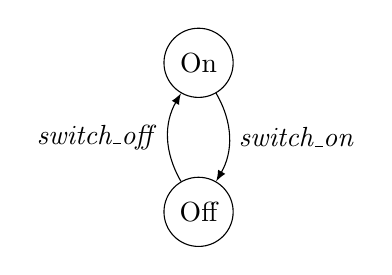
\begin{tikzpicture}
      \tikzstyle{every state}=[draw]

      \node[state] (on) {On};
      \node[state, below = of on] (off) {Off};

      \path (on)    edge[bend left] node {\emph{switch\_on}}  (off)
            (off)   edge[bend left] node {\emph{switch\_off}} (on);
      
    \end{tikzpicture}

    \caption{Simple automata \label{fig:deterministic_on}}
  \end{subfigure}
  ~
  \begin{subfigure}[b]{.45\textwidth}
    \centering
    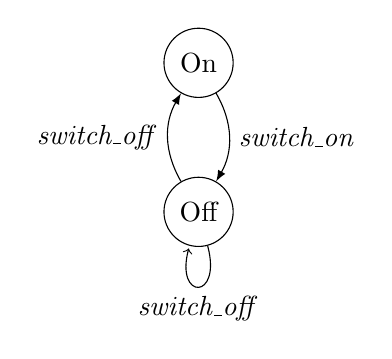
\begin{tikzpicture}
      \tikzstyle{every state}=[draw]
      
      \node[state] (on) {On};
      \node[state, below = of on] (off) {Off};
      
      \path (on)    edge[bend left]   node {\emph{switch\_on}}  (off)
      (off)   edge[bend left]   node {\emph{switch\_off}} (on)
      edge[loop below]  node {\emph{switch\_off}} (off);
      
    \end{tikzpicture}
    
    \caption{Non-deterministic automata \label{fig:non-deterministic_on}}
  \end{subfigure}
\end{figure}
Sometimes we have a non-deterministic behaviour \autoref{fig:non-deterministic_on}. We can go
to two different states coming from the same previous state and having the same input

\subsection{Definition of a labelled transition system}

Definition
\textbf{This is a test}


\subsection{Transition system with an infinite state space}

Example: the natural numbers

\begin{align*}
  S &= \{ 0, 1, 2, 3, ... \} \\
  Act &= \{ Up, Down \}  \\
  \rightarrow &= \{ <i, Up, i+1>, <i, Down, i-1> \}
\end{align*}

If we were to remove the transition from 2 and 3 we would have unreachable states



% !TEX root = ../main.tex

\section{Graph metrics}

What is essential on the graph?

Types of properties:
\begin{enumerate}
  \item Local: property of the surrounding node
  \item Global: characteristic of the entire graph
\end{enumerate}

\subsection{Graph metrics}
\subsubsection{Degree}

Degree $d_j$ of node $j$: number of neighbours of $j$

\begin{figure}
  \centering
  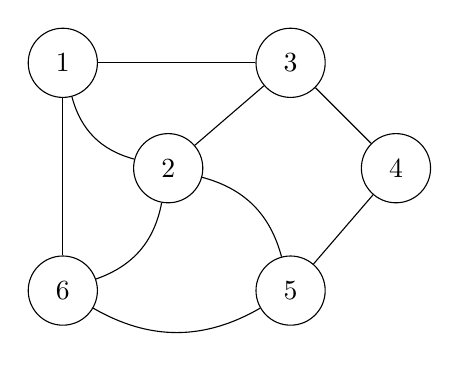
\begin{tikzpicture}
    \node[state] (1) {1};
    \node[state, right = 2 of 1] (3) {3};
    \node[state, below right = of 1] (2) {2};
    \node[state, below right = of 3] (4) {4};
    \node[state, below = 2 of 1] (6) {6};
    \node[state, below = 2 of 3] (5) {5};

    \draw[-]    (1)   edge    (3)
                      edge[bend right]    (2)
                      edge    (6)
                (2)   edge[bend left]     (6)
                      edge[bend left]     (5)
                      edge    (3)
                (5)   edge    (4)
                      edge[bend left]     (6)
                (4)   edge    (3);
                    
  \end{tikzpicture}
\end{figure}

$$
\sum_{j=1}^N d_j = 2L
$$

Average degree in $\mathcal{G}$ equals:
$$
E[D] = \frac{1}{N} \sum_{j=1}^N d_j = \frac{2L}{N}
$$

Bounds (connected graph):
$$
2 - \frac{2}{N} \le E[D] \le N-1
$$

$$
L(K_N) = 
\begin{pmatrix}
  N \\ 2
\end{pmatrix} = \frac{N (N-1)}{2}
$$

Degree vector (row sum A): $d = Au$
\begin{itemize}
  \item Coordinate representation of the vector: $u = (1, 1, ..., 1)$
  \item Matrix representation of the vector $u^T = [1 1 ... 1]$. A vector in $m$ dimensions is
  a $m \times 1$ matrix (elements in a column)
\end{itemize}

\emph{Basic law of the degree}:
$$
u^T d = 2L \xRightarrow{thus} u^Td = u^T Au = 2L
$$

\begin{itemize}
  \item At least two nodes in G have the same degree
  \begin{itemize}
    \item A degree $N-1$ node excludes the existence of a zero degree node
  \end{itemize}
  \item The number of nodes with \textbf{odd} degree is \textbf{even}
\end{itemize}

You can also create a histogram plotting all the degrees. This allows you to have the average
and the variance of the degrees (slide 6).

Example: degree of an airport
The probability is almost linear in a log scale. It has been found that many real life problems
have an almost linear degree distribution.
$$
Pr[D_{\text{Air}} = k] \sim k^{-1.21}
$$

Internet:
$$
Pr[D_{\text{Internet}} = k] \sim k^{-\tau}, \quad \tau \in (2.2, 2.5)
$$

Many networks have a power law degree distribution (scale-free networks)

\subsubsection{Clustering coefficient}
The degree can be seen as a global metric. This one goes a bit step further.

The clustering coefficient of node $v$ is 
$$
c_G(v) = \frac{2y}{d_v(d_v - 1)} = \frac{y}{y_{max}}
$$

where $y$ is the number of links between neighbors and 
$
y_{max} = \begin{pmatrix}
  d_v \\ 2
\end{pmatrix}
$

This number tells you how connected your environment is. The clustering coefficient of a graph G:
$$
c_G = \frac{1}{N} \sum_{v = 1}^N c_G(v)
$$

\subsubsection{Adjacency matrix A and walks}
\begin{itemize}
  \item Walk of length $k$ from node $i$ to $j$: succession of $k$ links (arcs)
  $n_0 \rightarrow n_1)(n_1 \rightarrow n_2) ... (n_{k-1} \rightarrow n_k)$ where $n_0 = i$ and
  $n_k = j$.
  \item Path: a walk in which all nodes/vertices are different
  \item Number of $k$-hop walks between node $i$ and $j$: $(A^k)_{ij}$
  \item Total number of $k$-hop walks in G: $N_k = u^T A^k u = \sum_{i=1}^N \sum_{j=1}^N (A^k)_{ij}$
  \item Total number of closed $k$-hop walks in G:
  $$
  W_k = \sum_{j=1}^N (A^k)_{jj} = \text{trace}(A^k)
  $$
\end{itemize}

\subsubsection{Weight of a path P}
Consider a weighted graph, where each link $l$ has a link weight $w_l$.

The weight of a path P is defined as:
$$
w(P) = \sum_{l \in P} w_l
$$

where $l = n_i \rightarrow n_j$ is a link in $G$ from node $n_i$ to $n_j$ and part of the path
$P = (n_0 \rightarrow n_1)(n_01 \rightarrow n_2)...(n_i \rightarrow n_j)...(n_{h-1} \rightarrow n_h)$
The path $P = P_{n_0 \rightarrow n_h}$ from node $n_0$ to $n_h$ consists of $h$ \emph{different, 
consecutive} links

\subsubsection{Hopcount}
\begin{itemize}
  \item Hopcount of a path $P$ is $h(P) = \sum_{l \in P} 1$, this link weight $w_l = 1$. 
  \item Hopcount from node $i$ to node $j$: 
  $H_{i \rightarrow j} = \min_{P_{i \rightarrow j}} h(P_{i \Rightarrow j}) 
  = h(P_{i \rightarrow j}^{*})$ where $P_{i \rightarrow j}^*$ is the shortest hop path from
  $i$ to $j$
  \item Number of $k$-hop walks between node $i$ and $j$: $(A^k)_{ij}$
\end{itemize}

Algebraic algorithm to find the shortest path
$$
\begin{pmatrix}
  (A)_{ij} = 0 \\
  (A^2)_{ij} = 0 \\
  \vdots \\
  (A^{k -1})_{ij} = 0 \\
  (A^k)_{ij} = m > 0
\end{pmatrix}
$$

The sequence tells us that there are no walks between $i$ and $j$ with less than $k$ hops.

Hence: the shortest walk between $i$ and $j$ is also a shortest path, with hopcount $H_{ij} = k$

There are $m$ different shortest paths with $k$ hops

\subsubsection{Hopcount \& Distance matrix}
A distance matrix $H$ satisfies vector norm or distance relations:
\begin{enumerate}
  \item $h_{ij} \ge 0$
  \item zero diagonal elements: $h_{ij} = 0$
  \item triangle inequality: $h_{ik} + h_{kj} \ge h_{ij}$
\end{enumerate}

\textbf{Diameter} $\rho$: 
\begin{itemize}
  \item Sequence with most zeros (or maximum $k$)
  \item All elements in $\sum_{k =0}^{\rho} f_k A^k$ with all $f_k > 0$ are positive
\end{itemize}

Choose $f_k = \begin{pmatrix}
  \rho \\ k
\end{pmatrix} > 0$
then $\sum_{k = 0}^{\rho} \begin{pmatrix}
  \rho \\ k
\end{pmatrix} A^k = (I + A)^{\rho}$.

The \textbf{small world problem}:
\begin{itemize}
  \item 160 letters: 1 target (name, address, occupation, personal info)
  \item 160 random starters
  \item Each starter forwards a letter to a single acquaintance
  \item Outcome experiment: Average hops of path = 6: everybody is connected by (on average) 6 hops.
\end{itemize}

\subsubsection{Betweenness}

The betweenness $B_l(B_n)$ of a link $l$ (node $n$) equals the number of shortest paths traversink
link $l$ (node $n$) in $G$).

The average betweenness is related to the average hopcount:
$$
H_G = \sum_{i = 1}^N \sum_{j = i + 1}^N H_{ij} = \sum_{l = 1}^L B_l
\implies
E[B_l] = \frac{1}{L} \sum_{l = 1}^L B_l = \frac{1}{L}
\begin{pmatrix}
  N \\ 2
\end{pmatrix}
E[H_G] \ge E[H_G]
$$

If there are many shortest paths we need to adjust the definition. If there are $k$ shortest
paths you count each one of them as $\frac{1}{k}$ 

\subsubsection{Linear correlation coefficient}
Consider $n$ realizations $\{(x_i, y_i)\}_{1 \le i\le m}$ of two random variables $X$ and $Y$.

Goodness of the fit can be expressed by the linear correlation coefficient
$$
\rho(X, Y) = \frac{E[XY] - E[X]E[Y]}{\sqrt{Var[X]}\sqrt{Var[Y]}}
$$

\begin{itemize}
  \item $\rho(X,Y) = 0$: No linear correlation
  \item $\rho(X, Y) = 1$: Perfect fit
\end{itemize}

\subsubsection{Degree assortativity}

Correlation between the left part of the link and the right part. How are the degrees $D_i$ 
and $D_j$ at both sides of a link $l$ correlated?

\begin{itemize}
  \item A network is assortative if $\rho_D > 0$
  \item A network is disassortative if $\rho_D < 0$
\end{itemize}

$$
\rho_D = \frac{N_1 N_3 - N_2^2}{N_1 \sum_{j=1}^N d_j^3 - N_2^2}
$$

Where $N_k = u^T A^k u$ is the total number of walks with $k$ hops

\subsubsection{Degree preserving rewiring}
Between two pairs of nodes you keep the degree, however you rewire the network, and, by doing
that you change the shape of the network and the connectivity. How many rewiring do you have to 
make in order to change the network from assortative to disassortative?

\subsubsection{Connectivity of the complement $G^C$}
If the graph G is disconnected, then ist complement $G^C$ is connected


% !TEX root = ../main.tex

\section{Spectrum}

\subsection{Eigenvalues and eigenvectors}

$$
Ax = \lambda x
$$

\begin{itemize}
  \item An eigenvector $x$ is a non-zero vector belonging to eigenvalue $\lambda$
  \item An $n \times n$ matrix $A$ has $n$ eigenvalues (possibly not all distinct)
  \item The eigenvalue problem for the transposed matrix leads us to talk about 
  right-eigenvectors ($A$ and $A^T$ have the same eigenvalues, but not necessarily the same
  eigenvectors) 
  \item The eigenvectors are linearly independent
  \item Mostly, we normalized eigenvectors such that $x^Tx = 1$
  \item If $P^{-1}$ exists, then $PAP^{-1}$ has the same eigenvalues as $A$, but each 
  eigenvector is $y = Px$, where $x$ is an eigenvector of $A$
\end{itemize}

\begin{align*}
  A(rx) = \lambda (rx) \quad r \ne 1
\end{align*}

\begin{gather*}
  A 
  \begin{bmatrix}
    x_1 & x_2 & \cdots & x_N
  \end{bmatrix} =
  \begin{bmatrix}
    x_1 & x_2 & \cdots & x_N
  \end{bmatrix}
  \begin{bmatrix}
    \lambda_1 & & & \\
    & \lambda_2 & & \\
    & & \ddots & \\
    & & & \lambda_N
  \end{bmatrix} \\
  AX = X\Lambda \implies A = X\Lambda X^{-1} \\
  (A - \lambda I)x = 0 \implies \det(A - \lambda I) = 0
\end{gather*}

\subsubsection{Basic theorem for symmetric matrices}
\textbf{Any real symmetric matrix $S$} can be written as $S = X \Lambda X^T$,
where $X$ is the orthogonal matrix with real eigenvectors in the columns and 
$\Lambda = diag(\lambda_1, ..., \lambda_N)$, where $\lambda_j$ is the $j$-th real eigenvalue.

The real eigenvalues can be ordered as

\begin{gather*}
  \lambda_N \le \lambda_{N-1} \le \cdots \lambda_2 \le \lambda_1
\end{gather*}

If symmetric: $A = A^T = X \Lambda X^T = \sum_{k=1}^{N} \lambda_k x_k x^T_k$

\subsubsection{The orthogonal matrix X of a symmetric matrix A}

$$
A^T = \sum_{k=1}^N \lambda_k^m x_k x^T_k
$$

Orthogonality of eigenvectors: $x_k^T x_m = \delta_{km} \implies X^T X = I \implies X^{-1} = X^T$

A matrix and its inverse commute: $X^{-1}X = X X^{-1} \implies X^TX = XX^T = I$ \textbf{Double
orthogonality}. Both column vectors (=eigenvectors of A) and row vectors of $X$ are orthogonal.

\subsubsection{Gerschgorin's theorem}

It explains why we use spectral radious..

\begin{quotation}
  Each eigenvalue of an $n\times n$ matrix $A$ lies in at least one of the circular discs
  with a center $a_{jj}$ and radii $R_j = \sum_{k=1;k \ne j}^n |a_{jk}|$
\end{quotation}

\textbf{Consequence for Adjacency matrix $A$: } $|\lambda| \le \sum_{k=1}^n a_{rk} = d_r$
$$
\lambda_1 \le d_{max}
$$

The largest eigenvalue is always smaller thant the maximum degree

\textbf{Properties}:
\begin{itemize}
  \item Spectrum of $A$:
  \begin{itemize}
    \item All eigenvalues lie in the interval $(-d_{max}, d_{max}]$
    \item $\sum_{j=1}^N \lambda_j = 0 \qquad \sum_{j=1}^N \lambda_j^2 = 2L \qquad
    \sum_{j=1}^N \lambda_j^k = Trace(A^k)$
    \item Perron-Frobenius Theorem: $\lambda_1$ non-negative and components eigenvector $x_1$ are
    non-negative. (irreducible = connected: positive)
  \end{itemize}
  \item Spectrum of $Q = \Delta - A = BB^T$:
  \begin{itemize}
    \item Any eigenvalue $\mu_k$ is non-negative and the smallest $\mu_N = 0$
    \item Complexity (number of spanning trees is) $\epsilon(G) = \frac{1}{N} \prod_{k=1}^{N-1} \mu_k$
    \item The second smallest eigenvalue of the Laplacian $Q$, called \textbf{the algebraic 
    connectivity} $a(G) = \mu_{N-1}$, quantifies how strongly a graph is 
  \end{itemize}
\end{itemize}





\end{document}